% unit: u28
% sources: sources/016-exam-2.txt, sources/111-mit18-06scf11-ex2-pdf-download-file.txt, sources/112-mit18-06scf11-ex2s-pdf-download-file.txt
\section{Exam 2}\label{sec:u28}

The second unit exam tests Sections~\ref{sec:u16}--\ref{sec:u24} through four problems:
determinants of matrices built from orthonormal vectors, a least-squares line, projections
and the next Gram--Schmidt vector, and a determinant that is a polynomial in one repeated
entry. Each problem is restated below and solved with the reasoning an examiner wants to see,
followed by further practice problems of the same kind. Try each problem before reading its
solution.

\subsection{The exam problems}

\begin{example}[Determinants from orthonormal vectors]\label{ex:u28-q}
Let $\vb{q}_1,\vb{q}_2,\vb{q}_3$ be orthonormal vectors in $\R^{3}$ and
$Q=\begin{bmatrix}\vb{q}_1&\vb{q}_2&\vb{q}_3\end{bmatrix}$. Find all possible values of
(a) $\det Q$; (b) $\det\begin{bmatrix}\vb{q}_1+\vb{q}_2&\vb{q}_2+\vb{q}_3&\vb{q}_3+\vb{q}_1\end{bmatrix}$;
(c) $\det Q$ times $\det\begin{bmatrix}\vb{q}_2&\vb{q}_3&\vb{q}_1\end{bmatrix}$.

(a) $Q\T Q=I$, so $(\det Q)^{2}=\det Q\T\det Q=\det I=1$ and $\det Q=\pm1$. Both values occur:
$Q=I$ gives $+1$, and $Q=\operatorname{diag}(1,1,-1)$ gives $-1$.

(b) The new columns are combinations of the old ones:
\[
  \begin{bmatrix}\vb{q}_1+\vb{q}_2&\vb{q}_2+\vb{q}_3&\vb{q}_3+\vb{q}_1\end{bmatrix}
  =Q\,M,\qquad M=\begin{bmatrix} 1&0&1\\ 1&1&0\\ 0&1&1\end{bmatrix},
\]
since column $j$ of $QM$ is $Q$ times column $j$ of $M$. Expanding along the first row,
$\det M=1\cdot(1-0)-0+1\cdot(1-0)=2$, so the determinant is $\det Q\det M=\pm2$.
Linearity in each column gives the same answer: of the eight determinants obtained by
splitting every column, all but two have a repeated column and vanish, leaving
$\det[\vb{q}_1\;\vb{q}_2\;\vb{q}_3]+\det[\vb{q}_2\;\vb{q}_3\;\vb{q}_1]=2\det Q$ by part (c).

(c) $[\vb{q}_2\;\vb{q}_3\;\vb{q}_1]$ is $Q$ with its columns cycled, which takes two
exchanges (swap columns~1 and~2, then columns~2 and~3). An even number of exchanges keeps the
determinant, so the product is $(\det Q)^{2}=1$, whichever sign $\det Q$ has.
\end{example}

\begin{example}[A least-squares line through 21 points]\label{ex:u28-21}
Measurements are taken at the $21$ times $t=-10,-9,\dots,9,10$. All are $b_i=0$ except
$b=1$ at the middle time $t=0$. (a) Find the least-squares line $C+Dt$. (b) Onto which
subspace is $\vb{b}$ projected? Give a basis, and a nonzero vector perpendicular to it.

(a) Exact fitting would require the $21$ equations $C+Dt_i=b_i$, that is
$A\vb{x}=\vb{b}$ with $\vb{x}=(C,D)$ and $A$ the $21\times2$ matrix whose columns are
$\vb{1}=(1,\dots,1)$ and $\vb{t}=(-10,\dots,10)$. The normal equations need
\[
  \vb{1}\T\vb{1}=21,\qquad \vb{1}\T\vb{t}=\sum t_i=0,\qquad
  \vb{t}\T\vb{t}=2(1^{2}+2^{2}+\dots+10^{2})=2\cdot385=770,
\]
and $A\T\vb{b}=(\vb{1}\T\vb{b},\vb{t}\T\vb{b})=(1,0)$, since the only nonzero $b_i$ sits at
$t=0$. So
\[
  \begin{bmatrix} 21&0\\ 0&770\end{bmatrix}\begin{bmatrix}\hat C\\ \hat D\end{bmatrix}
  =\begin{bmatrix} 1\\ 0\end{bmatrix},\qquad \hat C=\frac1{21},\quad \hat D=0 .
\]
The best line is the horizontal line $y=\tfrac1{21}$ (Figure~\ref{fig:u28-21}). Because the
times are symmetric about $0$, the two columns of $A$ are orthogonal and the normal equations
uncouple: $\hat C$ is the average of the $b_i$, and $\hat D=\vb{t}\T\vb{b}/\vb{t}\T\vb{t}=0$.
A symmetric data set cannot prefer an upward or a downward slope.

(b) $\vb{b}\in\R^{21}$ is projected onto the column space of $A$, a plane in $\R^{21}$ with
basis $\vb{1}$ and $\vb{t}$. The error vector is perpendicular to it:
\[
  \vb{e}=\vb{b}-\vb{p}=\vb{b}-\tfrac1{21}\vb{1}=\tfrac1{21}(\underbrace{-1,\dots,-1}_{10},\,20,\,\underbrace{-1,\dots,-1}_{10}).
\]
Check: its components add to $\tfrac1{21}(20-20)=0$, and $\vb{t}\T\vb{e}=0$ by symmetry. A
simpler perpendicular vector is $(1,-2,1,0,\dots,0)$: its components add to $0$, and against
$\vb{t}$ it gives $-10+18-8=0$.
\end{example}

\begin{figure}[ht]\centering
\begin{tikzpicture}
\begin{axis}[width=0.75\textwidth,height=0.3\textwidth,xmin=-10.8,xmax=10.8,ymin=-0.15,ymax=1.15,
  axis lines=middle,xlabel={$t$},xtick={-10,-5,5,10},ytick={1},
  xlabel style={anchor=west},clip=false]
  \addplot[only marks,mark=*,mark size=1.6pt] coordinates {(-10,0) (-9,0) (-8,0) (-7,0) (-6,0)
    (-5,0) (-4,0) (-3,0) (-2,0) (-1,0) (0,1) (1,0) (2,0) (3,0) (4,0) (5,0) (6,0) (7,0) (8,0)
    (9,0) (10,0)};
  \addplot[blue,thick,domain=-10.5:10.5] {1/21};
  \node[blue,above,font=\small] at (axis cs:6,0.05) {$y=\tfrac1{21}$};
  \node[right,font=\small] at (axis cs:0.2,1) {$b=1$ at $t=0$};
\end{axis}
\end{tikzpicture}
\caption{The data of Example~\ref{ex:u28-21} and its least-squares line. Twenty points sit
at $0$ and one at $1$; the best line is the horizontal line at the average height
$\tfrac1{21}$. Any tilt would help on one side of $t=0$ exactly as much as it hurts on the
other.}
\label{fig:u28-21}
\end{figure}

\begin{example}[Projections from Gram--Schmidt and the next vector]\label{ex:u28-gs}
Gram--Schmidt turns independent vectors $\vb{a}_1,\vb{a}_2,\vb{a}_3$ in $\R^{5}$ into
orthonormal $\vb{q}_1,\vb{q}_2,\vb{q}_3$. Let $A$ and $Q$ be the $5\times3$ matrices with
these columns. (a) Give formulas for the projection matrices $P_A$ and $P_Q$ onto their
column spaces. (b) Is $P_Q=P_A$? What is $P_QQ$? What is $\det P_Q$? (c) A fourth vector
$\vb{a}_4$ is added, with $\vb{a}_1,\dots,\vb{a}_4$ independent. Which of these is the next
Gram--Schmidt vector $\vb{q}_4$?
\[
  \text{(1)}\ \frac{P_Q\vb{a}_4}{\|P_Q\vb{a}_4\|},\qquad
  \text{(2)}\ \frac{\vb{w}}{\|\vb{w}\|}\ \text{with}\
  \vb{w}=\vb{a}_4-\frac{\vb{a}_4\T\vb{a}_1}{\vb{a}_1\T\vb{a}_1}\vb{a}_1
  -\frac{\vb{a}_4\T\vb{a}_2}{\vb{a}_2\T\vb{a}_2}\vb{a}_2
  -\frac{\vb{a}_4\T\vb{a}_3}{\vb{a}_3\T\vb{a}_3}\vb{a}_3,\qquad
  \text{(3)}\ \frac{\vb{a}_4-P_A\vb{a}_4}{\|\vb{a}_4-P_A\vb{a}_4\|}.
\]

(a) $P_A=A(A\T A)^{-1}A\T$ and $P_Q=Q(Q\T Q)^{-1}Q\T=QQ\T$, because $Q\T Q=I$.

(b) Yes, $P_Q=P_A$. Gram--Schmidt never leaves the span: each $\vb{q}_j$ is a combination
of $\vb{a}_1,\dots,\vb{a}_j$ and each $\vb{a}_j$ a combination of $\vb{q}_1,\dots,\vb{q}_j$,
so $\Col{Q}=\Col{A}$, and the projection onto a subspace depends only on the subspace, not on
the basis used to describe it. (Substituting $A=QR$ into $A(A\T A)^{-1}A\T$ and cancelling
also works.) Next, $P_QQ=QQ\T Q=Q$: vectors already in the subspace are not moved. Finally
$\det P_Q=0$: $P_Q$ is $5\times5$ with rank $3$, and every vector perpendicular to $\Col{Q}$ is
sent to $\vb{0}$.

(c) Choice (3). The vector $\vb{a}_4-P_A\vb{a}_4$ is the error of projecting $\vb{a}_4$ onto
$\Col{A}$, so it is perpendicular to $\vb{q}_1,\vb{q}_2,\vb{q}_3$; it is nonzero because
$\vb{a}_4$ is not in $\Col{A}$; dividing by its length makes it a unit vector. This is
exactly what Gram--Schmidt computes, usually written
$\vb{a}_4-(\vb{q}_1\T\vb{a}_4)\vb{q}_1-(\vb{q}_2\T\vb{a}_4)\vb{q}_2-(\vb{q}_3\T\vb{a}_4)\vb{q}_3$.
Choice (1) is the projection itself, which lies \emph{in} the old subspace, the opposite of
what we want. Choice (2) is the tempting one: it would be right with the orthogonal
$\vb{q}_i$ in place of the $\vb{a}_i$, but subtracting projections onto lines that are not
perpendicular to each other does not leave a vector perpendicular to all of them.
\end{example}

The failure of choice (2) is easy to see in a small case. In $\R^{3}$ take
$\vb{a}_1=(1,0,0)$, $\vb{a}_2=(1,1,0)$ and a new vector $\vb{a}_3=(1,1,1)$. The formula of
choice (2) gives
$\vb{w}=(1,1,1)-\tfrac11(1,0,0)-\tfrac22(1,1,0)=(-1,0,1)$, and $\vb{w}\cdot\vb{a}_1=-1\neq0$.
The correct $\vb{a}_3-P_A\vb{a}_3$ is $(0,0,1)$, perpendicular to the whole plane of
$\vb{a}_1,\vb{a}_2$.

\begin{example}[A determinant that is a polynomial]\label{ex:u28-poly}
A $4\times4$ matrix has the same number $x$ in every position of its first row and first
column (the exam writes $\times$ for it); the other nine entries are fixed numbers.
(a) $\det A$ is a polynomial in $x$. What is its largest possible degree? (b) If the nine
numbers form the $3\times3$ identity, find $\det A$ and the values of $x$ that make it zero.

(a) Degree at most $2$. Each term of the big formula takes exactly one entry from each row
and each column. All the $x$'s lie in row~1 or column~1, so a term can contain at most one
$x$ from row~1 and at most one from column~1; the corner entry $a_{11}=x$ uses up both. So
each term has at most two factors $x$. Part (b) shows the degree $2$ is actually reached.

(b) The matrix is
\[
  A=\begin{bmatrix} x&x&x&x\\ x&1&0&0\\ x&0&1&0\\ x&0&0&1\end{bmatrix}.
\]
Subtract $x$ times rows~2, 3 and~4 from row~1; this does not change the determinant and
clears the last three entries of row~1, leaving $x-3x^{2}$ in the corner. The result is
lower triangular, so
\[
  \det A=(x-3x^{2})\cdot1\cdot1\cdot1=x(1-3x).
\]
It is zero for $x=0$ (a zero row) and for $x=\tfrac13$. For $x=\tfrac13$ the dependence is
visible: rows~2, 3, 4 add to $(1,1,1,1)$, which is $3$ times row~1.
\end{example}

\begin{trap}
In Example~\ref{ex:u28-poly}(a) it is tempting to count the seven $x$'s and guess degree $7$,
or to count four per row and guess $4$. The big formula is the right tool for questions about
the \emph{form} of a determinant: one entry per row and per column limits how many $x$'s can
meet in one term.
\end{trap}

\subsection{Further practice}

\begin{exercise}\label{exr:u28-q2}
With $\vb{q}_1,\vb{q}_2,\vb{q}_3$ orthonormal in $\R^{3}$, find the determinants
\[
  \det\begin{bmatrix}\vb{q}_1-\vb{q}_2&\vb{q}_2-\vb{q}_3&\vb{q}_3-\vb{q}_1\end{bmatrix}
  \qquad\text{and}\qquad
  \det\begin{bmatrix}\vb{q}_1+\vb{q}_2&\vb{q}_1-\vb{q}_2&\vb{q}_3\end{bmatrix}.
\]
\end{exercise}
\begin{solution}
The three columns of the first matrix add to $\vb{0}$, so they are dependent and the
determinant is $0$. For the second, write it as $QM$ with
$M=\left[\begin{smallmatrix} 1&1&0\\ 1&-1&0\\ 0&0&1\end{smallmatrix}\right]$;
$\det M=1\cdot(-1)-1\cdot1=-2$, so the determinant is $-2\det Q=\mp2$. Geometrically, the
first two columns are perpendicular with length $\sqrt2$ each, so the box has volume
$\sqrt2\cdot\sqrt2\cdot1=2$, in agreement with the volume interpretation of Section~\ref{sec:u22}.
\end{solution}

\begin{exercise}\label{exr:u28-5pts}
Measurements at $t=-2,-1,0,1,2$ are $\vb{b}=(0,0,0,0,1)$. Find the least-squares line
$C+Dt$ and check that the error is perpendicular to both columns of $A$.
\end{exercise}
\begin{solution}
The columns $\vb{1}$ and $\vb{t}=(-2,-1,0,1,2)$ are orthogonal, with $\vb{1}\T\vb{1}=5$ and
$\vb{t}\T\vb{t}=10$; also $\vb{1}\T\vb{b}=1$ and $\vb{t}\T\vb{b}=2$. So $\hat C=\tfrac15$ and
$\hat D=\tfrac2{10}=\tfrac15$: the line is $y=\tfrac15(1+t)$. Its values at the five times are
$\vb{p}=\tfrac15(-1,0,1,2,3)$, so $\vb{e}=\vb{b}-\vb{p}=\tfrac15(1,0,-1,-2,2)$. Check:
$1+0-1-2+2=0$ and $-2+0+0-2+4=0$. Unlike Example~\ref{ex:u28-21}, the lone nonzero
measurement is off-centre, so the line tilts toward it.
\end{solution}

\begin{exercise}\label{exr:u28-poly2}
Repeat Example~\ref{ex:u28-poly}(b) when the nine numbers form $2I$ instead of $I$.
\end{exercise}
\begin{solution}
Subtract $\tfrac{x}{2}$ times rows~2, 3, 4 from row~1. The corner becomes
$x-3\cdot\tfrac{x}{2}\cdot x=x-\tfrac32x^{2}$, the rest of row~1 becomes $0$, and the
remaining diagonal is $2,2,2$. So $\det A=8\bigl(x-\tfrac32x^{2}\bigr)=8x-12x^{2}=4x(2-3x)$,
which vanishes for $x=0$ and $x=\tfrac23$. The degree is again $2$, as part (a) of the
example predicts.
\end{solution}
